\documentclass[mstat,12pt]{unswthesis}


\usepackage{array}
\usepackage{calc}
\usepackage{enumitem}
\usepackage{svg}
\usepackage{color}
\usepackage{fancyvrb}
\newcommand{\VerbBar}{|}
\newcommand{\VERB}{\Verb[commandchars=\\\{\}]}
\DefineVerbatimEnvironment{Highlighting}{Verbatim}{commandchars=\\\{\}}
% Add ',fontsize=\small' for more characters per line
\usepackage{framed}
\definecolor{shadecolor}{RGB}{248,248,248}
\newenvironment{Shaded}{\begin{snugshade}}{\end{snugshade}}
\newcommand{\AlertTok}[1]{\textcolor[rgb]{0.94,0.16,0.16}{#1}}
\newcommand{\AnnotationTok}[1]{\textcolor[rgb]{0.56,0.35,0.01}{\textbf{\textit{#1}}}}
\newcommand{\AttributeTok}[1]{\textcolor[rgb]{0.13,0.29,0.53}{#1}}
\newcommand{\BaseNTok}[1]{\textcolor[rgb]{0.00,0.00,0.81}{#1}}
\newcommand{\BuiltInTok}[1]{#1}
\newcommand{\CharTok}[1]{\textcolor[rgb]{0.31,0.60,0.02}{#1}}
\newcommand{\CommentTok}[1]{\textcolor[rgb]{0.56,0.35,0.01}{\textit{#1}}}
\newcommand{\CommentVarTok}[1]{\textcolor[rgb]{0.56,0.35,0.01}{\textbf{\textit{#1}}}}
\newcommand{\ConstantTok}[1]{\textcolor[rgb]{0.56,0.35,0.01}{#1}}
\newcommand{\ControlFlowTok}[1]{\textcolor[rgb]{0.13,0.29,0.53}{\textbf{#1}}}
\newcommand{\DataTypeTok}[1]{\textcolor[rgb]{0.13,0.29,0.53}{#1}}
\newcommand{\DecValTok}[1]{\textcolor[rgb]{0.00,0.00,0.81}{#1}}
\newcommand{\DocumentationTok}[1]{\textcolor[rgb]{0.56,0.35,0.01}{\textbf{\textit{#1}}}}
\newcommand{\ErrorTok}[1]{\textcolor[rgb]{0.64,0.00,0.00}{\textbf{#1}}}
\newcommand{\ExtensionTok}[1]{#1}
\newcommand{\FloatTok}[1]{\textcolor[rgb]{0.00,0.00,0.81}{#1}}
\newcommand{\FunctionTok}[1]{\textcolor[rgb]{0.13,0.29,0.53}{\textbf{#1}}}
\newcommand{\ImportTok}[1]{#1}
\newcommand{\InformationTok}[1]{\textcolor[rgb]{0.56,0.35,0.01}{\textbf{\textit{#1}}}}
\newcommand{\KeywordTok}[1]{\textcolor[rgb]{0.13,0.29,0.53}{\textbf{#1}}}
\newcommand{\NormalTok}[1]{#1}
\newcommand{\OperatorTok}[1]{\textcolor[rgb]{0.81,0.36,0.00}{\textbf{#1}}}
\newcommand{\OtherTok}[1]{\textcolor[rgb]{0.56,0.35,0.01}{#1}}
\newcommand{\PreprocessorTok}[1]{\textcolor[rgb]{0.56,0.35,0.01}{\textit{#1}}}
\newcommand{\RegionMarkerTok}[1]{#1}
\newcommand{\SpecialCharTok}[1]{\textcolor[rgb]{0.81,0.36,0.00}{\textbf{#1}}}
\newcommand{\SpecialStringTok}[1]{\textcolor[rgb]{0.31,0.60,0.02}{#1}}
\newcommand{\StringTok}[1]{\textcolor[rgb]{0.31,0.60,0.02}{#1}}
\newcommand{\VariableTok}[1]{\textcolor[rgb]{0.00,0.00,0.00}{#1}}
\newcommand{\VerbatimStringTok}[1]{\textcolor[rgb]{0.31,0.60,0.02}{#1}}
\newcommand{\WarningTok}[1]{\textcolor[rgb]{0.56,0.35,0.01}{\textbf{\textit{#1}}}}


%%%%%%%%%%%%%%%%%%%%%%%%%%%%%%%%%%%%%%%%%%%%%%%%%%%%%%%%%%%%%%%%%%
% 
% OK...Now we get to some actual input.  The first part sets up
% the title etc that will appear on the front page
%
%%%%%%%%%%%%%%%%%%%%%%%%%%%%%%%%%%%%%%%%%%%%%%%%%%%%%%%%%%%%%%%%%

\title{Projet réalisé par\\[0.5cm] l'équipe TDDT du groupe de TD1 \\[3cm]Rapport
de groupe des UE \newline  Bases de données + Sciences des Données 2}

\authornameonly{ }

\author{
  \begin{tabular}{c}
  MOUTCHACHOU Lydia \\
  IBNMTAR Hazem \\
  BERETTI--PRENANT Esteban \\
  VAROL Serdar
  \end{tabular}
}

\copyrightfalse
\figurespagefalse
\tablespagefalse

%%%%%%%%%%%%%%%%%%%%%%%%%%%%%%%%%%%%%%%%%%%%%%%%%%%%%%%%%%%%%%%%%
%
%  And now the document begins
%  The \beforepreface and \afterpreface commands puts the
%  contents page etc in
%
%%%%%%%%%%%%%%%%%%%%%%%%%%%%%%%%%%%%%%%%%%%%%%%%%%%%%%%%%%%%%%%%%%


%%%%%%%%%%%%%%%%%%%%%%%%%%%%%%%%%%%%%%%%%%%%%%%%%%%%%%%%%%%%%%%%%%%%%%%
%
%  A small sample UNSW Coursework Masters thesis file.
%  Any questions to Ian Doust i.doust@unsw.edu.au and/or Gery Geenens ggeenens@unsw.edu.au
%
%%%%%%%%%%%%%%%%%%%%%%%%%%%%%%%%%%%%%%%%%%%%%%%%%%%%%%%%%%%%%%%%%%%%%%%
%
%  The first part pulls in a UNSW Thesis class file.  This one is
%  slightly nonstandard and has been set up to do a couple of
%  things automatically
%
 
%%%%%%%%%%%%%%%%%
%% Precisely one of the next four lines should be uncommented.
%% Choose the one which matches your degree, uncomment it, and comment out the other two!
%\documentclass[mfin,12pt]{unswthesis}    %%  For Master of Financial Mathematics 
%\documentclass[mmath,12pt]{unswthesis}   %%  For Master of Mathematics
%\documentclass[mstat,12pt]{unswthesis}  %%  For Master of Statistics
%%%%%%%%%%%%%%%%%



\linespread{1}
\usepackage{amsfonts}
\usepackage{amssymb}
\usepackage{amsthm}
\usepackage{latexsym,amsmath}
\usepackage{graphicx}
\usepackage{afterpage}
\usepackage[colorlinks]{hyperref}
 \hypersetup{
     colorlinks=true,
     linkcolor=blue,
     filecolor=blue,
     citecolor= black,      
     urlcolor=cyan,
     }
\usepackage{textcomp}
\usepackage{longtable}
\usepackage{booktabs}
\usepackage{float}
\let\origfigure\figure
\let\endorigfigure\endfigure
\renewenvironment{figure}[1][2] {
    \expandafter\origfigure\expandafter[H]
} {
    \endorigfigure
}
\usepackage[T1]{fontenc}
\usepackage{ragged2e}
\def\tightlist{}
\usepackage[french]{babel}

%%%%%%%%%%%%%%%%%%%%%%%%%%%%%%%%%%%%%%%%%%%%%%%%%%%%%%%%%%%%%%%%%
%
%  The following are some simple LaTeX macros to give some
%  commonly used letters in funny fonts. You may need more or less of
%  these
%
\newcommand{\R}{\mathbb{R}}
\newcommand{\Q}{\mathbb{Q}}
\newcommand{\C}{\mathbb{C}}
\newcommand{\N}{\mathbb{N}}
\newcommand{\F}{\mathbb{F}}
\newcommand{\PP}{\mathbb{P}}
\newcommand{\T}{\mathbb{T}}
\newcommand{\Z}{\mathbb{Z}}
\newcommand{\B}{\mathfrak{B}}
\newcommand{\BB}{\mathcal{B}}
\newcommand{\M}{\mathfrak{M}}
\newcommand{\X}{\mathfrak{X}}
\newcommand{\Y}{\mathfrak{Y}}
\newcommand{\CC}{\mathcal{C}}
\newcommand{\E}{\mathbb{E}}
\newcommand{\cP}{\mathcal{P}}
\newcommand{\cS}{\mathcal{S}}
\newcommand{\A}{\mathcal{A}}
\newcommand{\ZZ}{\mathcal{Z}}
%%%%%%%%%%%%%%%%%%%%%%%%%%%%%%%%%%%%%%%%%%%%%%%%%%%%%%%%%%%%%%%%%%%%%
%
% The following are much more esoteric commands that I have left in
% so that this file still processes. Use or delete as you see fit
%
\newcommand{\bv}[1]{\mbox{BV($#1$)}}
\newcommand{\comb}[2]{\left(\!\!\!\begin{array}{c}#1\\#2\end{array}\!\!\!\right)
}
\newcommand{\Lat}{{\rm Lat}}
\newcommand{\var}{\mathop{\rm var}}
\newcommand{\Pt}{{\mathcal P}}
\def\tr(#1){{\rm trace}(#1)}
\def\Exp(#1){{\mathbb E}(#1)}
\def\Exps(#1){{\mathbb E}\sparen(#1)}
\newcommand{\floor}[1]{\left\lfloor #1 \right\rfloor}
\newcommand{\ceil}[1]{\left\lceil #1 \right\rceil}
\newcommand{\hatt}[1]{\widehat #1}
\newcommand{\modeq}[3]{#1 \equiv #2 \,(\text{mod}\, #3)}
\newcommand{\rmod}{\,\mathrm{mod}\,}
\newcommand{\p}{\hphantom{+}}
\newcommand{\vect}[1]{\mbox{\boldmath $ #1 $}}
\newcommand{\reff}[2]{\ref{#1}.\ref{#2}}
\newcommand{\psum}[2]{\sum_{#1}^{#2}\!\!\!'\,\,}
\newcommand{\bin}[2]{\left( \begin{array}{@{}c@{}}
				#1 \\ #2
			\end{array}\right)	}
%
%  Macros - some of these are in plain TeX (gasp!)
%
\newcommand{\be}{($\beta$)}
\newcommand{\eqp}{\mathrel{{=}_p}}
\newcommand{\ltp}{\mathrel{{\prec}_p}}
\newcommand{\lep}{\mathrel{{\preceq}_p}}
\def\brack#1{\left \{ #1 \right \}}
\def\bul{$\bullet$\ }
\def\cl{{\rm cl}}
\let\del=\partial
\def\enditem{\par\smallskip\noindent}
\def\implies{\Rightarrow}
\def\inpr#1,#2{\t \hbox{\langle #1 , #2 \rangle} \t}
\def\ip<#1,#2>{\langle #1,#2 \rangle}
\def\lp{\ell^p}
\def\maxb#1{\max \brack{#1}}
\def\minb#1{\min \brack{#1}}
\def\mod#1{\left \vert #1 \right \vert}
\def\norm#1{\left \Vert #1 \right \Vert}
\def\paren(#1){\left( #1 \right)}
\def\qed{\hfill \hbox{$\Box$} \smallskip}
\def\sbrack#1{\Bigl \{ #1 \Bigr \} }
\def\ssbrack#1{ \{ #1 \} }
\def\smod#1{\Bigl \vert #1 \Bigr \vert}
\def\smmod#1{\bigl \vert #1 \bigr \vert}
\def\ssmod#1{\vert #1 \vert}
\def\sspmod#1{\vert\, #1 \, \vert}
\def\snorm#1{\Bigl \Vert #1 \Bigr \Vert}
\def\ssnorm#1{\Vert #1 \Vert}
\def\sparen(#1){\Bigl ( #1 \Bigr )}

\newcommand\blankpage{%
    \null
    \thispagestyle{empty}%
    \addtocounter{page}{-1}%
    \newpage}

%%%%%%%%%%%%%%%%%%%%%%%%%%%%%%%
%
% These environments allow you to get nice numbered headings
%  for your Theorems, Definitions etc.  
%
%  Environments
%
%%%%%%%%%%%%%%%%%%%%%%%%%%%%%%%

\newtheorem{theorem}{Theorem}[section]
\newtheorem{lemma}[theorem]{Lemma}
\newtheorem{proposition}[theorem]{Proposition}
\newtheorem{corollary}[theorem]{Corollary}
\newtheorem{conjecture}[theorem]{Conjecture}
\newtheorem{definition}[theorem]{Definition}
\newtheorem{example}[theorem]{Example}
\newtheorem{remark}[theorem]{Remark}
\newtheorem{question}[theorem]{Question}
\newtheorem{notation}[theorem]{Notation}
\numberwithin{equation}{section}

%%%%%%%%%%%%%%%%%%%%%%%%%%%%%%%%%%%%%%%%%%%%%%%%%%%%%%%%%%%%%%%%%%
%
%  If you've got some funny special words that LaTeX might not
% hyphenate properly, you can give it a helping hand:
%

\hyphenation{Mar-cin-kie-wicz Rade-macher}


\newlength{\cslhangindent}
\setlength{\cslhangindent}{1.5em}
\newlength{\csllabelwidth}
\setlength{\csllabelwidth}{3em}
\newenvironment{CSLReferences}[2] % #1 hanging-ident, #2 entry spacing
 {% don't indent paragraphs
  \setlength{\parindent}{0pt}
  % turn on hanging indent if param 1 is 1
  \ifodd #1 \everypar{\setlength{\hangindent}{\cslhangindent}}\ignorespaces\fi
  % set entry spacing
  \ifnum #2 > 0
  \setlength{\parskip}{#2\baselineskip}
  \fi
 }%
 {}
\usepackage{calc} % for \widthof, \maxof
\newcommand{\CSLBlock}[1]{#1\hfill\break}
\newcommand{\CSLLeftMargin}[1]{\parbox[t]{\maxof{\widthof{#1}}{\csllabelwidth}}{#1}}
\newcommand{\CSLRightInline}[1]{\parbox[t]{\linewidth}{#1}}
\newcommand{\CSLIndent}[1]{\hspace{\cslhangindent}#1}






\renewcommand{\contentsname}{Table des matières}

\renewcommand{\chaptername}{Chapitre}




\begin{document}

\beforepreface

%\afterpage{\blankpage}

% plagiarism

\prefacesection{Déclaration de non plagiat}

\textcolor{red}{À compléter avant la remise du rapport.}

\vskip 2pc \noindent Nous déclarons que ce rapport est le fruit de notre seul travail, à part lorsque cela est indiqué  explicitement. 

\vskip 2pc  \noindent Nous acceptons que la personne évaluant ce rapport puisse, pour les besoins de cette évaluation:
\begin{itemize}
\item la reproduire et en fournir une copie à un autre membre de l'université; et/ou,
\item en communiquer une copie à un service en ligne de détection de plagiat (qui pourra en retenir une copie pour les besoins d'évaluation future).
\end{itemize}

\vskip 2pc \noindent Nous certifions que nous avons lu et compris les règles ci-dessus.\vspace{24pt}

\vskip 2pc \noindent En signant cette déclaration, nous acceptons ce qui précède.
\vskip 2pc \noindent
Signature: \rule{7cm}{0.25pt} \hfill Date: \rule{4cm}{0.25pt} \\[1cm]
\vskip 1pc

%\textcolor{red}{Mettre à jour la date.}

{\bigskip\bigskip\bigskip\noindent} \today
%\afterpage{\blankpage}

% Acknowledgements are optional


\prefacesection{Remerciements}

\textcolor{red}{À compléter avant la remise du rapport.}

{\bigskip}Nos plus sincères remerciements vont à notre encadrant
pédagogique pour les conseils avisés sur notre travail.\\[1cm] Nous
remercions aussi \ldots{}\\[1cm] 

{\bigskip\bigskip\bigskip\noindent} \today

%\afterpage{\blankpage}

% Abstract

\prefacesection{Résumé}

Notre projet vise à analyser les performances financières des
entreprises françaises entre 2018 et 2022 à partir des données du
Registre National du Commerce et des Sociétés (RNCS). Nous cherchons à
comprendre quels sont les facteurs qui influencent la rentabilité des
entreprises et comment ces dernières évoluent en fonction de leur
secteur d'activité. Plus précisément, nous allons : - Comparer les
performances des entreprises selon leur chiffre d'affaires et leur
rentabilité. - Étudier l'impact de la fiscalité sur la profitabilité des
entreprises. - Analyser l'évolution des ventes, des stocks et des taxes
pour identifier des tendances économiques.

%\afterpage{\blankpage}


\afterpreface





%%%%%%%%%%%%%%%%%%%%%%%%%%%%%%%%%%%%%%%%%%%%%%%%%%%%%%%%%%%%%%%%%%
%
% Now we can start on the first chapter
% Within chapters we have sections, subsections and so forth
%
%%%%%%%%%%%%%%%%%%%%%%%%%%%%%%%%%%%%%%%%%%%%%%%%%%%%%%%%%%%%%%%%%%



%%%%%%%%%%%%%%%%%%%%%%%%%%%%%%%%%%%%%

%\afterpage{\blankpage}


\chapter{Introduction}\label{introduction}

\section{Présentation du projet}\label{pruxe9sentation-du-projet}

Les données financières des entreprises jouent un rôle crucial dans la
compréhension de leur santé économique. Ce projet se concentre sur
l'analyse des performances financières des entreprises françaises entre
2018 et 2022, en utilisant les données fournies par le Registre National
du Commerce et des Sociétés (RNCS).

\bigskip

\begin{itemize}[label=$\circ$]
    \item \textbf{Comparer les performances des entreprises selon leur chiffre d'affaires et leur rentabilité.}
    \item \textbf{Étudier l’impact de la fiscalité sur la profitabilité des entreprises.}
    \item \textbf{Analyser l’évolution des ventes, des stocks et des taxes pour identifier des tendances économiques.}
\end{itemize}

\medskip

\section{Responsabilités et composition de
l'équipe}\label{responsabilituxe9s-et-composition-de-luxe9quipe}

\medskip

MOUTCHACHOU Lydia : Étudiant n°22212656

IBNMTAR Hazem : Étudiant n°22309227

BERETTI--PRENANT Esteban : Étudiant n°22208752

VAROL Serdar : Étudiant n°22009668

\bigskip

\section{Objectifs et questions de
recherche}\label{objectifs-et-questions-de-recherche}

Notre projet vise à analyser les performances financières des
entreprises françaises entre 2018 et 2022. Pour ce faire, nous allons
examiner plusieurs facteurs qui pourraient influencer la rentabilité des
entreprises. Les questions spécifiques que nous allons aborder sont les
suivantes :

\subsection{\texorpdfstring{\textbf{Comparaison de la rentabilité par
rapport au chiffre d'affaires
:}}{Comparaison de la rentabilité par rapport au chiffre d'affaires :}}\label{comparaison-de-la-rentabilituxe9-par-rapport-au-chiffre-daffaires}

\begin{enumerate}
\def\labelenumi{\alph{enumi}.}
\item
  Comment la rentabilité varie-t-elle en fonction de la taille de
  l'entreprise ?
\item
  Y a-t-il une différence notable entre les entreprises qui ont recours
  au refinancement et celles qui n'en ont pas besoin ?
\end{enumerate}

\subsection{\texorpdfstring{\textbf{Comparaison de la rentabilité par
rapport au
chiffre}}{Comparaison de la rentabilité par rapport au chiffre}}\label{comparaison-de-la-rentabilituxe9-par-rapport-au-chiffre}

\begin{enumerate}
\def\labelenumi{\alph{enumi}.}
\item
  La rentabilité des entreprises diffère-t-elle selon la ville où elles
  sont implantées ?
\item
  Les entreprises qui exportent leurs produits ou services sont-elles
  plus rentables que celles qui opèrent uniquement sur le marché
  national ?
\end{enumerate}

\subsection{\texorpdfstring{\textbf{Impact fiscal et sectoriel
:}}{Impact fiscal et sectoriel :}}\label{impact-fiscal-et-sectoriel}

\begin{enumerate}
\def\labelenumi{\alph{enumi}.}
\item
  Quel est l'impact des taxes sur la rentabilité des entreprises ?
\item
  Comment la rentabilité varie-t-elle selon le secteur d'activité des
  entreprises ?
\end{enumerate}

\subsection{\texorpdfstring{\textbf{Évolution temporelle
:}}{Évolution temporelle :}}\label{uxe9volution-temporelle}

\begin{enumerate}
\def\labelenumi{\alph{enumi}.}
\item
  Comment la rentabilité des entreprises a-t-elle évolué entre 2012 et
  2016 ?
\item
  Peut-on identifier des tendances spécifiques ou des périodes de
  croissance/déclin dans les performances financières des entreprises ?
\end{enumerate}

\medskip

En répondant à ces questions, nous espérons identifier les principaux
facteurs influençant la rentabilité des entreprises françaises et
fournir des insights précieux pour les décideurs économiques et les
gestionnaires d'entreprises.

\chapter{Base de données}\label{base-de-donnuxe9es}

\section{Provenance des données}\label{provenance-des-donnuxe9es}

Les données utilisées dans ce projet proviennent du jeu de données
Kaggle : \medskip

\begin{itemize}[label=$\circ$]
  \item \textnormal{\textbf{Profit and loss \- Ontology.csv :} Contient les comptes de résultat de 100 000 entreprises françaises, avec des informations détaillées sur les revenus, les dépenses et les bénéfices.}
  
  \item \textnormal{\textbf{APE\_Fusion.csv :} Utilise le code APE pour classer les entreprises selon leur secteur d’activité, permettant des comparaisons sectorielles précises.}

  \item \textnormal{\textbf{Data\_Kaggle.csv :} Fournit des données globales sur les entreprises, incluant les ventes, les stocks et les taxes, permettant d'analyser l’évolution des performances financières sur plusieurs années.}
\end{itemize}

\medskip

\textit{Lien vers les données :}
\href{https://www.kaggle.com/datasets/briaclg/financial-data-of-french-compagnies/data?select=Profit+and+loss+-+Onthology.csv}{Kaggle Dataset}

\section{Descriptif des tables}\label{descriptif-des-tables}

\bigskip

\subsection{Table 1: APE\_Fusion.csv}\label{table-1-ape_fusion.csv}

\begin{table}[H]
\centering
\scriptsize
\begin{tabular}{|p{3.2cm}|p{1.2cm}|p{7.5cm}|p{2.5cm}|}
\hline
\textbf{Nom colonne} & \textbf{Type} & \textbf{Signification} & \textbf{Caractéristique} \\
\hline
Unname d: 0 & int & Index ou identifiant de ligne (peut être ignoré dans l'analyse) & \\
\hline
ape & object & Code APE complet de l'activité principale de l'entreprise & Clé primaire \\
\hline
ape\_name & object & Nom ou description de l'activité correspondant au code APE & \\
\hline
ape\_len & int & Longueur du code APE, indiquant le nombre de caractères qu'il contient & \\
\hline
ape\_cat0 & int & Premier niveau du code APE (division), composé des 2 premiers chiffres & \\
\hline
ape\_cat1 & float & Deuxième niveau du code APE (groupe), composé des 3 premiers chiffres & \\
\hline
ape\_cat2 & float & Troisième niveau du code APE (classe), composé des 4 premiers chiffres & \\
\hline
ape\_cat3 & object & Dernier niveau du code APE (sous-classe) & \\
\hline
Libellé & object & Description du secteur d'activité auquel appartient le code APE & \\
\hline
Code & object & Code alphabétique supplémentaire associé au secteur d'activité & \\
\hline
\end{tabular}
\footnotesize
\label{tab:ape_description}
\end{table}

\subsection{Table 2 : Profit and loss -
Ontology.csv}\label{table-2-profit-and-loss---ontology.csv}

\begin{table}[H]
\centering
\scriptsize
\begin{tabular}{|p{4cm}|p{2cm}|p{9cm}|}
\hline
\textbf{Nom colonne} & \textbf{Type} & \textbf{Signification} \\
\hline
Columns\_(FR/EN) & varchar & Colonnes des états financiers en français et en anglais \\
\hline
Description (FR) & varchar & Explication de ce que chaque colonne représente \\
\hline
Liasse (Id) & int & Identifiant unique des colonnes dans la base INPI \\
\hline
Calcul & varchar & Méthode de calcul pour certaines valeurs dans les colonnes \\
\hline
\end{tabular}
\normalsize
\end{table}

\subsection{Table 3 : Data\_Kaggle.csv}\label{table-3-data_kaggle.csv}

\scriptsize
\begin{longtable}{|p{0.7cm}|p{12cm}|p{1.5cm}|}
\hline
\textbf{N\textdegree} & \textbf{Variable} & \textbf{Code} \\
\hline \endfirsthead
\hline \textbf{N\textdegree} & \textbf{Variable Nome} & \textbf{Nome de Colon} \\ \hline \endhead
1 & year & B \\
2 & Autres imp\^ots, taxes et versements assimil\'es & C \\
3 & Ventes de marchandises & D \\
4 & Production vendue biens & E \\
5 & Production vendue services & F \\
6 & Chiffres d\'affaires nets & G \\
7 & Production stock\'ee & H \\
8 & Production immobilis\'ee & I \\
9 & Subventions d\'exploitation & J \\
10 & Reprises sur amortissements et provisions, transfert de charges & K \\
11 & Autres produits & L \\
12 & Total des produits d\'exploitation & M \\
13 & Achats de marchandises (y compris droits de douane) & N \\
14 & Variation de stock (marchandises) & O \\
15 & Achats de mati\`eres premi\`eres et autres approvisionnements & P \\
16 & Variation de stock (mati\`eres premi\`eres et approvisionnements) & Q \\
17 & Autres achats et charges externes & R \\
18 & Imp\^ots, taxes et versements assimil\'es & S \\
19 & Salaires et traitements & T \\
20 & Charges sociales & U \\
21 & Autres charges & V \\
22 & Total des charges d\'exploitation & W \\
23 & R\'esultat d'exploitation & X \\
24 & B\'en\'efice attribu\'e ou perte transf\'er\'ee & Y \\
25 & Perte support\'ee ou b\'en\'efice transf\'er\'e & Z \\
26 & Produits financiers de participations & AA \\
27 & Produits des autres valeurs mobili\`eres et cr\'eances de l\'actif immobilis\'e & AB \\
28 & Autres int\'er\^ets et produits assimil\'es & AC \\
29 & Reprises sur provisions et transferts de charges financier & AD \\
30 & Diff\'erences positives de change & AE \\
31 & Produits nets sur cessions de valeurs mobili\`eres de placement & AF \\
32 & Total des produits financiers & AG \\
33 & Dotations financi\`eres sur amortissements et provisions & AH \\
34 & Int\'er\^ets et charges assimil\'ees & AI \\
35 & Diff\'erences n\'egatives de change & AJ \\
36 & Charges nettes sur cessions de valeurs mobili\`eres de placement & AK \\
37 & Total des charges financi\`eres & AL \\
38 & R\'esultat financier & AM \\
39 & R\'esultat en cours avant imp\^ots & AN \\
40 & Produits exceptionnels sur op\'erations de gestion & AO \\
41 & Produits exceptionnels sur op\'erations en capital & AP \\
42 & Reprises sur provisions et transferts de charges exceptionnel & AQ \\
43 & Total des produits exceptionnels & AR \\
44 & Charges exceptionnelles sur op\'erations de gestion & AS \\
45 & Charges exceptionnelles sur op\'erations en capital & AT \\
46 & Dotations exceptionnelles aux amortissements et provisions & AU \\
47 & Total des charges exceptionnelles & AV \\
48 & R\'esultat exceptionnel & AW \\
49 & Participation des salari\'es aux r\'esultats de l\'entreprise & AX \\
50 & Imp\^ots sur les b\'en\'efices & AY \\
51 & Total des produits & AZ \\
52 & Total des charges & BA \\
53 & B\'en\'efices ou perte (Total des produits - Total des charges) & BB \\
54 & Imp\^ots diff\'er\'es (compte de r\'esultat) & BC \\
55 & R\'esultat net des soci\'et\'es mises en \'equivalence & BD \\
56 & R\'esultat net des entreprises int\'egr\'ees & BE \\
57 & R\'esultat Groupe (R\'esultat net consolid\'e) & BF \\
58 & Part des int\'er\^ets minoritaires (R\'esultat hors groupe) & BG \\
59 & R\'esultat net part du groupe (part de la soci\'et\'e m\`ere) & BH \\
60 & R\'emun\'eration d\'interm\'ediaires et honoraires (hors r\'etrocessions) & BI \\
61 & Location, charges locatives et de copropri\'et\'e & BJ \\
62 & Effectif moyen du personnel & BK \\
63 & Sous-traitance & BL \\
64 & Personnel ext\'erieur \`a l\'entreprise & BM \\
65 & R\'etrocessions d\'honoraires, commissions et courtages & BN \\
66 & Taxe professionnelle & BO \\
67 & Montant de la TVA. collect\'ee & BP \\
\hline
\end{longtable}
\normalsize
\scriptsize
\begin{longtable}{|p{0.7cm}|p{12cm}|p{1.5cm}|}
\hline
\textbf{N\textdegree} & \textbf{Variable} & \textbf{Code} \\
\hline \endfirsthead
\hline \textbf{N\textdegree} & \textbf{Variable Nome} & \textbf{Nome de Colon} \\ \hline \endhead
68 & Total TVA. d\'eductible sur biens et services & BQ \\
69 & Dividendes & BR \\
70 & siren & BS \\
\hline
\end{longtable}
\normalsize

\section{Modèles MCD et MOD}\label{moduxe8les-mcd-et-mod}

\begin{itemize}
\tightlist
\item
  Pour le MCD, inclure une image réalisée avec le logiciel Mocodo
  \href{https://www.mocodo.net/?mcd=eNqNksFu2zAMhu96Ch0dQAOW7Zab67ZK2zTL4ixtcjEUh14FOJKhyFm3N_J9b-AX62_HaOMEAwb4Ay1SIvlLjMvNQRmvrRnxWDsywe3DQPD43R296MwRCw9Wu7AgMRzy2Ka6rnxdieGUwyfJsKMZNUsBpmrX2kj5z50ddvZLZ7-Kid5QniNNZLfEMoXyTTWUC7OM3EWpLpggiq2j0BgixhyldLClQ8uC945wnPkQ0u1_D49auYJfk7E7fdwjeNNKYfde5WJhf8GBZtlM_SYXvSj380w_b7tq_Ena3lNX5KzT05u9DcE1kOAePIIp-AZm4DuYM3bzWljnyc2c3ZbaX9btAv3CSzJbR01Il_97pi-g12sMFuAHWIIn8AxWYC24_PNp9cxGDN9Z5pMsEiLlA5gAiJUQKyFWQuwYlzG-AhHApaxvBF8h-WrNIrsrvNroXHtqH79Z05z2Ze5VTxm_nA1xoVX866VO0_bEz-uqdfqEXovcavxhQgIpe7FMG2VSTS6Qy4H48Ktm6hK9K-q_fh_Ip7OEKRVNNkN5ML5DbGExcUlxbHkfjCcDcXSlbc_wPGLXVV2Zusp0SklBGI5gPB2wN-SeTJ4=}{https://www.moc\\odo.net}
  telle que celle visible sur la Figure\(~\)\ref{MCD} ci-dessous :
\end{itemize}

\begin{figure}
\centering
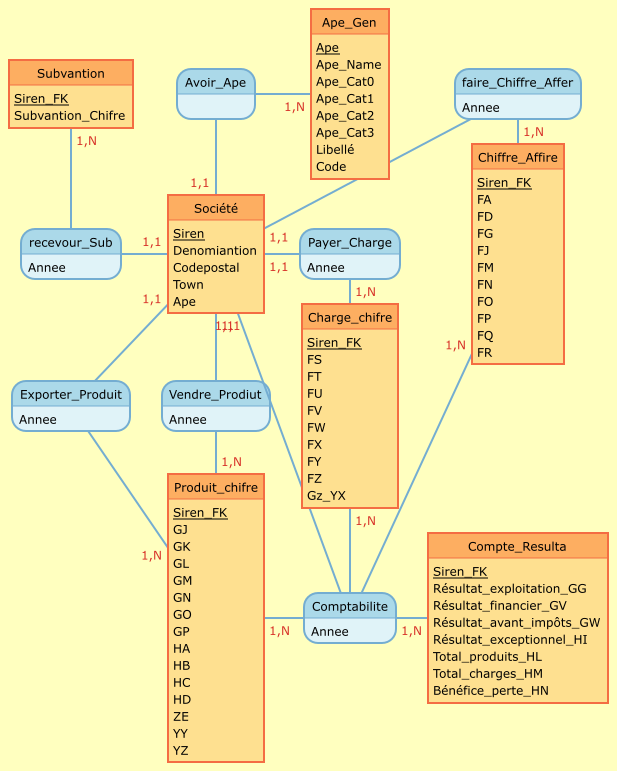
\includegraphics[width=8cm,height=10cm]{MCD.png}
\caption{MCD}\label{MCD}
\end{figure}

\begin{Shaded}
\begin{Highlighting}[]
\FunctionTok{getwd}\NormalTok{()}
\end{Highlighting}
\end{Shaded}

\begin{verbatim}
## [1] "/Users/serdarvarol/Desktop/PVL_L2-24_25/Project_DataBase_FR/template_2025/GroupReportTemplate 2"
\end{verbatim}

\begin{itemize}
\tightlist
\item
  Pour le MOD, inclure une image réalisée avec le designer de phpmyadmin
\end{itemize}

\bigskip

Noter en passant qu'il est possible de créer des diagrammes en R
Markdown au moyen du package \texttt{DiagrammeR}
{[}\url{https://rich-iannone.github.io/DiagrammeR/graphviz_and_mermaid.html}{]}
comme on peut le voir ci-dessous.

\begin{Shaded}
\begin{Highlighting}[]
\CommentTok{\# install.packages("webshot",dependencies = TRUE)}
\CommentTok{\# library(webshot)}
\CommentTok{\# webshot::install\_phantomjs()}
\FunctionTok{Sys.setenv}\NormalTok{(}\AttributeTok{OPENSSL\_CONF=}\StringTok{"/dev/null"}\NormalTok{)}
\NormalTok{DiagrammeR}\SpecialCharTok{::}\FunctionTok{grViz}\NormalTok{(}\StringTok{"}
\StringTok{digraph boxes\_and\_circles \{}

\StringTok{  \# a \textquotesingle{}graph\textquotesingle{} statement}
\StringTok{  graph [overlap = true, fontsize = 10]}

\StringTok{  \# several \textquotesingle{}node\textquotesingle{} statements}
\StringTok{  node [shape = box,}
\StringTok{        fontname = Helvetica]}
\StringTok{  A; B; C; D; E; F}

\StringTok{  node [shape = circle,}
\StringTok{        fixedsize = true,}
\StringTok{        width = 0.9] // sets as circles}
\StringTok{  1; 2; 3; 4; 5; 6; 7; 8}

\StringTok{  \# several \textquotesingle{}edge\textquotesingle{} statements}
\StringTok{  A{-}\textgreater{}1 B{-}\textgreater{}2 B{-}\textgreater{}3 B{-}\textgreater{}4 C{-}\textgreater{}A}
\StringTok{  1{-}\textgreater{}D E{-}\textgreater{}A 2{-}\textgreater{}4 1{-}\textgreater{}5 1{-}\textgreater{}F}
\StringTok{  E{-}\textgreater{}6 4{-}\textgreater{}6 5{-}\textgreater{}7 6{-}\textgreater{}7 3{-}\textgreater{}8}
\StringTok{\}}
\StringTok{"}\NormalTok{)}
\end{Highlighting}
\end{Shaded}

\section{Import des données}\label{import-des-donnuxe9es}

\begin{itemize}
\tightlist
\item
  Préciser les nettoyages réalisés avant l'import comme l'uniformisation
  des valeurs des champs (\emph{e.g.}, Mr, M., Monsieur, \ldots) ou le
  remplissage des valeurs manquantes par une valeur moyenne \ldots{}
\end{itemize}

\begin{itemize}
    \item  Source de données 1 :
    \begin{itemize} 
     \item Suppression des colonnes XXX, car XXX
     \item  Suppression des doublons dans les colonnes XXX
    \item  Filtrage en fonction de la colonne XXx, nous n'avons conservé que.... 
\end{itemize}
\end{itemize}

\section{Requêtes réalisées}\label{requuxeates-ruxe9alisuxe9es}

Pour chaque requête, l'exprimer en langage naturel puis en SQL. Puis
donner le résultat obtenu (ou un extrait) et expliquer ce résultat.

L'objectif est de varier le type de requêtes et de répondre à votre
problématique initiale.

\section{Quelques détails
techniques}\label{quelques-duxe9tails-techniques}

On peut interagir avec une base de données directement depuis RMarkdown.
Un fichier .Rmd sera fourni pour donner des exemples.

\chapter{Matériel et Méthodes}\label{matuxe9riel-et-muxe9thodes}

\section{Logiciels}\label{logiciels}

Lister tous les logiciels utilisé pour la partie statistique du rapport
(et également ceux pour gérer et communiquer entre les membres du projet
s'il y en a en particulier)

\medskip

R (ou Python) est le logiciel à privilégier pour la Science des Données.
Pour assurer une reproductibilité maximale, vous devriez utiliser R
Markdown (ou un Notebook Jupyter, et éventuellement un outil de gestion
des versions tel que \texttt{Git}), par exemple via Google Colab ou
RStudio dans les nuages. Évitez d'utiliser Word!

\bigskip

Il est de votre responsabilité de donner les versions des logiciels que
vous utilisez, ainsi que de donner des informations techniques sur
l'ordinateur qui vous a servi pour les analyses (système d'exploitation,
vitesse du processeur, etc.). Penser à fournir des citations pour les
logiciels utilisés, par exemple
\footnote{L'entrée BibTeX ajoutée dans le fichier \texttt{references.bib} a été obtenue grâce à la commande  \texttt{citation(package = "tidyverse")} tapée dans la console de R.}.

\section{Modélisation statistique}\label{moduxe9lisation-statistique}

Quels outils ou méthodes de statistiques allez-vous utiliser? Donner des
équations mathématiques s'il y a lieu et lister les éventuels
présupposés («assumptions» en anglais) que vous devez faire sur les
données afin d'utiliser ces outils ou méthodes (\emph{e.g.}, normalité,
absence de valeurs aberrantes, etc.).

Il est également bon d'indiquer quelles sont les avantages et les
limites de ces méthodes.

Vous pourrez consulter avec profit les Chapitre 11--13 du livre sur R
utilisé pendant le cours :

\url{http://biostatisticien.eu/springeR/livreR.pdf}

\chapter{Analyse Exploratoire des
Données}\label{analyse-exploratoire-des-donnuxe9es}

Toute étude impliquant des données doit \textbf{obligatoirement} inclure
une analyse exploratoire préalable. Celle-ci permet de mieux comprendre
l'information contenue dans les données.

Il faut produire de nombreux résumés graphiques (\emph{e.g.},
histogrammes, nuages de points, boxplots, etc.) et numériques
(\emph{e.g.}, médiane, moyenne, variance, etc.). Ainsi, il faut faire
une analyse descriptive uni- et bivariée systématique de toutes les
variables du jeu de données. Puis, il faut uniquement conserver les plus
pertinents (les autres pouvant être gardés en Annexe), c'est-à-dire ceux
qui permettront de dégager des éléments de réponse pour la question de
recherche envisagée. Chaque figure et tableau doit être commenté. Mais
il ne faut pas extrapoler et dire des choses qui ne sont pas visibles
dans ces graphiques ou tableaux. Pour chaque analyse, vous pourrez
préciser le nombre d'individus/ d'unités statistiques concernés au
total.

Vous pourrez consulter avec profit le Chapitre 9 du livre sur R utilisé
pendant le cours :

\url{http://biostatisticien.eu/springeR/livreR.pdf}

\section{Utiliser R}\label{utiliser-r}

Il est facile d'inclure des codes R dans votre rapport, qui seront
exécutés à la volée (\emph{i.e.}, lors de la traduction de votre fichier
\texttt{Rmd} en fichier \texttt{PDF} ou \texttt{DOC}). Par exemple:

\begin{Shaded}
\begin{Highlighting}[]
\FunctionTok{boxplot}\NormalTok{(cars, }\AttributeTok{col =} \FunctionTok{c}\NormalTok{(}\StringTok{"\#5975a4"}\NormalTok{, }\StringTok{"\#cc8963"}\NormalTok{))}
\end{Highlighting}
\end{Shaded}

\begin{figure}

{\centering 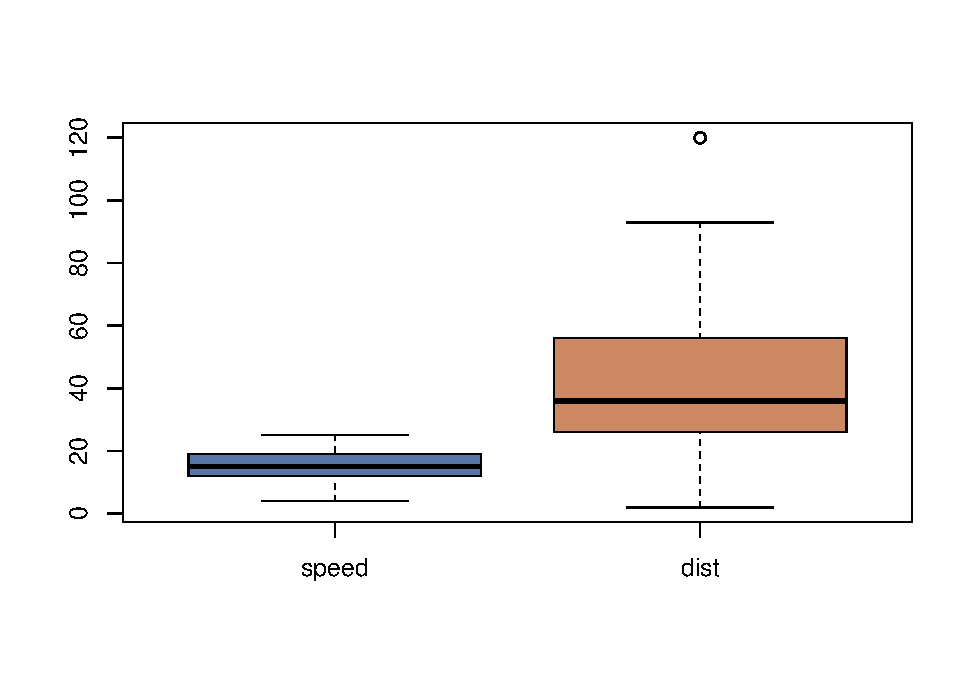
\includegraphics[width=7cm]{scdon2-UPV-report-template_sansPython_files/figure-latex/unnamed-chunk-3-1} 

}

\caption{\label{fig:boxplots}Deux boxplots.}\label{fig:unnamed-chunk-3}
\end{figure}

\begin{Shaded}
\begin{Highlighting}[]
\FunctionTok{colMeans}\NormalTok{(cars)}
\end{Highlighting}
\end{Shaded}

\begin{verbatim}
## speed  dist 
## 15.40 42.98
\end{verbatim}

Les lignes de code ne doivent pas dépasser dans la marge de droite.
Ainsi on pourrait remplacer le chunk ci-dessous:

\begin{Shaded}
\begin{Highlighting}[]
\FunctionTok{boxplot}\NormalTok{(cars, }\AttributeTok{main =} \StringTok{"Un titre qui est vraiment beaucoup trop long et qui dépasse dans la marge de droite"}\NormalTok{)}
\end{Highlighting}
\end{Shaded}

\begin{figure}

{\centering 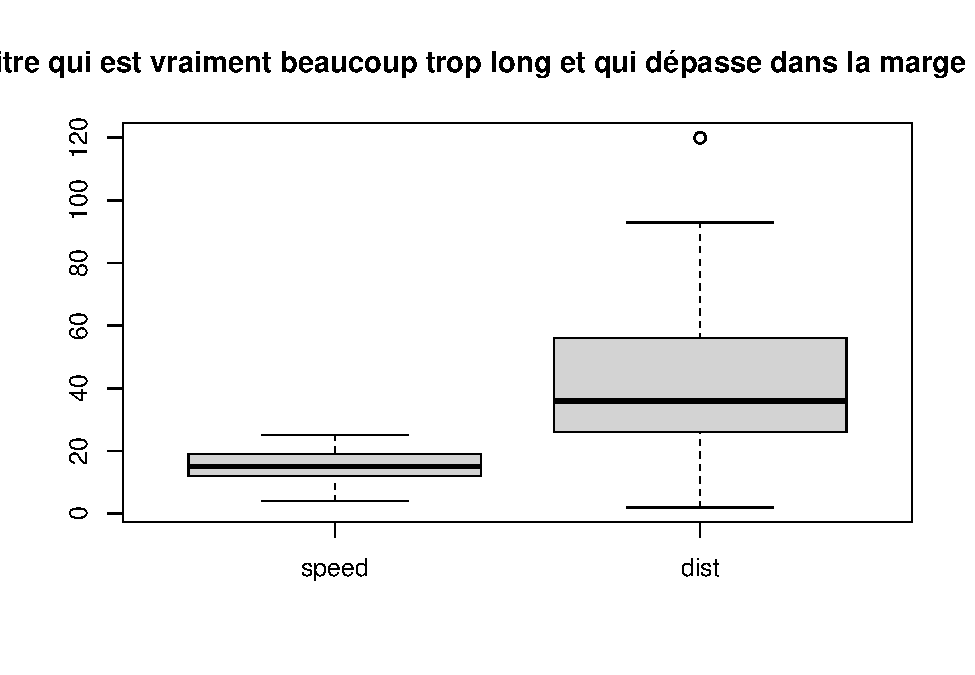
\includegraphics[width=7cm]{scdon2-UPV-report-template_sansPython_files/figure-latex/unnamed-chunk-4-1} 

}

\caption{Pas super.}\label{fig:unnamed-chunk-4}
\end{figure}

par celui-ci:

\tiny

\begin{Shaded}
\begin{Highlighting}[]
\FunctionTok{boxplot}\NormalTok{(cars, }
        \AttributeTok{main =} \StringTok{"Un titre qui est vraiment beaucoup trop long}\SpecialCharTok{\textbackslash{}n}\StringTok{ mais qui ne dépasse plus dans la marge de droite"}\NormalTok{)}
\end{Highlighting}
\end{Shaded}

\begin{figure}

{\centering 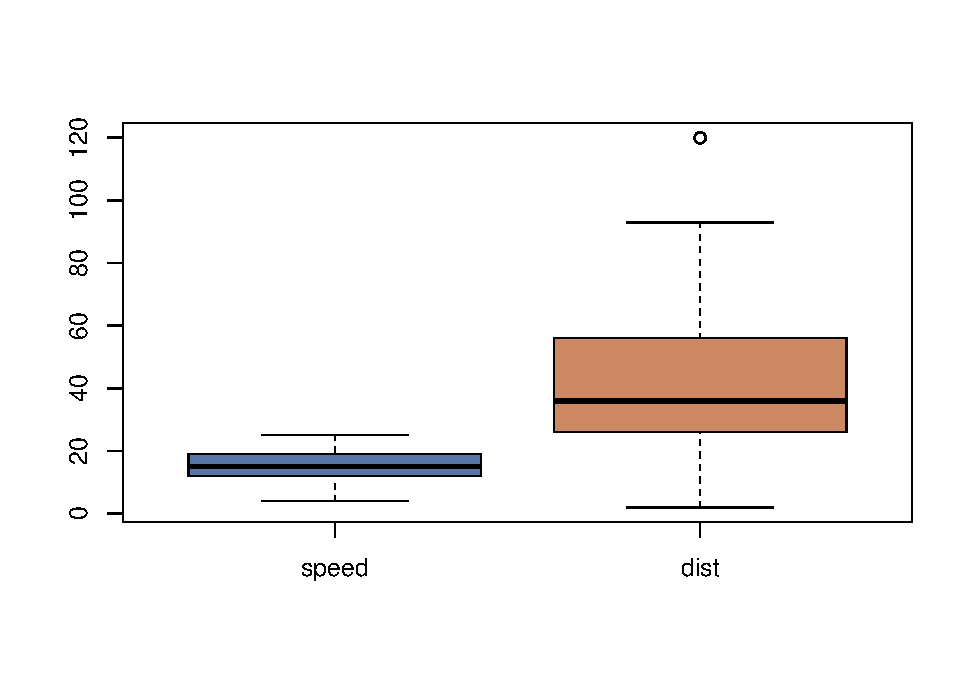
\includegraphics[width=7cm]{scdon2-UPV-report-template_sansPython_files/figure-latex/unnamed-chunk-5-1} 

}

\caption{Déjà mieux.}\label{fig:unnamed-chunk-5}
\end{figure}

\normalsize

où l'on a:

\begin{itemize}
\tightlist
\item
  utilisé la commande \LaTeX~\texttt{\textbackslash{}tiny} pour changer
  la taille de la police (suivi de de
  \texttt{\textbackslash{}normalsize} pour revenir à la taille normale),
\item
  mis l'instruction \texttt{main\ =\ ...} sur la deuxième ligne,
\item
  utilisé \texttt{\textbackslash{}n} pour afficher le titre sur deux
  lignes.
\end{itemize}

\chapter{Analyse et Résultats}\label{analyse-et-ruxe9sultats}

Dans cette partie, vous pourrez utiliser les outils et méthodes vus au
semestre précédent pour analyser les liens entre les variables.

Pour cela, vous pourrez utiliser les tests du \(\chi^2\), test du
coefficient de corrélation linéaire, test d'Anova, la droite de
régression linéaire.

Vous pourrez également proposer des modèles pour faire du clustering
(k-means, CAH), de la classification (K plus proches voisins par
exemple) comme vu en Science des données 1.

\section{La droite de régression linéaire : un premier
exemple}\label{la-droite-de-ruxe9gression-linuxe9aire-un-premier-exemple}

Si on souhaite expliquer les variations d'une variables réponse \(Y\) en
fonction d'un certain nombre de prédicteurs \(x_1,\ldots,x_p\), on peut
utiliser un modèle de régression linéaire simple (\(p=1\)) ou multiple
(\(p>1\))

\[
Y_i = \beta_0 + \beta_1 x_{1i} + \cdots +\beta_p x_{pi} + \epsilon_i, \qquad i=1,\ldots,n.
\] où l'on présuppose que les \(\epsilon_i\) sont i.i.d.~\(N(0,1)\) pour
tout \(i=1,\ldots,n\) (\(n\) étant la taille de l'échantillon).

Vous pourrez toujours consulter avec profit les Chapitre 11--13 du livre
sur R utilisé pendant le cours :

\url{http://biostatisticien.eu/springeR/livreR.pdf}

Ces chapitres détaillent l'utilisation de certains tests et modèles sous
\texttt{R}.

\chapter{Discussion}\label{discussion}

Placer les résultats que vous avez obtenus dans le chapitre précédent en
perspective par rapport au problème étudié.

\chapter{Conclusion et perspectives}\label{conclusion-et-perspectives}

Quelles sont les conclusions principales? Quelles sont vos
recommandations pour le commanditaire? Quelles analyses subséquentes
pourraient être faites dans le futur?

\bigskip

On attend de vous deux types de perspectives : des perspectives à court
terme pour améliorer rapidement votre approche et des perspectives à
plus long terme qu'elles soient liées à la science des données ou au
domaine métier pour lequel vous avez travaillé.

\bigskip

Lister également les difficultés rencontrées dans la partie BD (e.g.,
taille de la base, manque de données, \ldots) et dans la partie
statistique.

\chapter*{Bibliographie}\label{bibliographie}
\addcontentsline{toc}{chapter}{Bibliographie}

\phantomsection\label{refs}
\begin{CSLReferences}{0}{1}
\end{CSLReferences}

\bibliographystyle{elsarticle-harv}
\bibliography{references}

\chapter*{Annexes}\label{annexes}
\addcontentsline{toc}{chapter}{Annexes}

Il faut utiliser les annexes de façon judicieuse. C'est ici que l'on
place des résultats trop volumineux pour apparaître dans le corps du
rapport. Ou bien des résultats (e.g., graphiques) moins intéressants que
les autres. Cela permet de limiter le nombre de pages du coeur du
rapport, et d'ajouter des détails dans cette partie pour le lecteur
désireux d'en savoir plus.

\section*{\texorpdfstring{\textbf{Codes}}{Codes}}\label{codes}
\addcontentsline{toc}{section}{\textbf{Codes}}

Ajouter vos codes informatique ici. Les codes doivent être correctement
indentés et commentés.

\section*{\texorpdfstring{\textbf{Tables}}{Tables}}\label{tables}
\addcontentsline{toc}{section}{\textbf{Tables}}

Si vous avez des tableaux supplémentaires, vous pouvez les ajouter ici.

Utiliser \url{https://www.tablesgenerator.com/markdown_tables} pour
créer des tables Markdown simples, ou bien utiliser \LaTeX.

\begin{longtable}[]{@{}lcr@{}}
\caption{une légende au-dessus du tableau.
\label{tab7.1}}\tabularnewline
\toprule\noalign{}
Les tables & sont & cool \\
\midrule\noalign{}
\endfirsthead
\toprule\noalign{}
Les tables & sont & cool \\
\midrule\noalign{}
\endhead
\bottomrule\noalign{}
\endlastfoot
col 1 est & alignée à gauche & \$1600 \\
col 2 est & centrée & \$12 \\
col 3 est & alignée à droite & \$1 \\
\end{longtable}

Aligner les nombres de la troisième colonne sur la droite permet
d'afficher les unités au-dessus des unités, les dizaines au-dessus des
dizaines, etc. Il faut toujours privilégier cette présentation.







\end{document}

